\documentclass{article}[18pt]
\usepackage{tikz}
\usepackage{enumitem}


\begin{document}
\begin{center}
\underline{\huge ADS Coursework}
\end{center}
Suppose you want an output to be the list of length 8
$$[7,6,5,4,3,2,1,0]$$
For this to be the worst case for the merge, the two lists of length four to be merged should run out at the same time. So the lists should be List A: $[7,5,3,1]$ and List B: $[6,4,2,0]$.\\
\\
Selection sort has no worst case, as the same number of comparisons will be used for any list of a given length. So just for example, the input to selection sort is the numbers in ascending order, but those numbers could be in any order for a worst case of the algorithm.
\\
For these two sublists to be produced from a list of length 8, each half should be one of the sublists, so a worst case for a list of length 8 would be.
$$[1,3,5,6,0,2,4,6]$$
Below is a demonstration of the algorithm running on that input list
\begin{center}

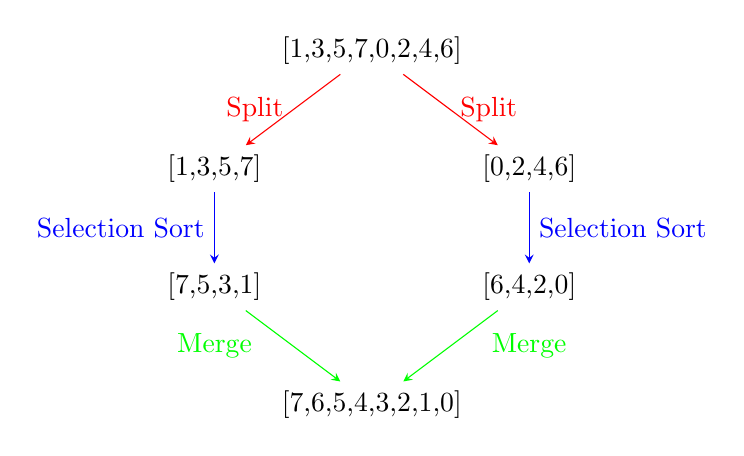
\begin{tikzpicture}[node distance=2cm]
\tikzstyle{arrow} = [->,>=stealth]

% nodes
\node (A) at (0, 0.5) {[1,3,5,7,0,2,4,6]};
\node (B) at (-2, -1) {[1,3,5,7]};
\node (C) at (2, -1) {[0,2,4,6]};
\node (D) at (-2, -2.5) {[7,5,3,1]};
\node (E) at (2, -2.5) {[6,4,2,0]};
\node (F) at (0, -4) {[7,6,5,4,3,2,1,0]};
% arrows

\draw [arrow,red] (A) -- node[anchor=east] {Split} (B);
\draw [arrow,red] (A) -- node[anchor=west] {Split} (C);
\draw [arrow,blue] (B) -- node[anchor=east] {Selection Sort} (D);
\draw [arrow,blue] (C) -- node[anchor=west] {Selection Sort} (E);
\draw [arrow,green] (D) -- node[anchor=east,xshift=-4mm] {Merge} (F);
\draw [arrow,green] (E) -- node[anchor=west,xshift=4mm] {Merge} (F);


\end{tikzpicture}

\end{center}

\end{document}